
\newcommand{\sagadocument}{ExTENCI: SAGA Condor Integration}
\newcommand{\sagaversion}{1.0-\textbf{DRAFT}}
\newcommand{\sagabasename}{saga-programming-guide}
\newcommand{\sagaemail}{\{oweidner|sjha\} @ cct.lsu.edu}

\documentclass{article}

\usepackage{ifpdf}

\ifpdf
  \usepackage[pdftex]{graphicx}
  \usepackage[pdftex]{hyperref}
  \DeclareGraphicsExtensions{.pdf, .png, .jpg}
  \graphicspath{{pics/}}
\else
  \usepackage{graphicx}
  \usepackage[hypertex]{hyperref}
  \DeclareGraphicsExtensions{.ps, .eps}
  \graphicspath{{pics/}}
\fi


\usepackage{srcltx}
\usepackage{fancyhdr}
\usepackage{wrapfig}
\usepackage{fancyvrb}
\usepackage{lscape}
\usepackage{color}
\usepackage{xspace}

\newcommand{\F}[1]{\textbf{#1}}
\newcommand{\B}[1]{\textbf{#1}}
\newcommand{\I}[1]{\textit{#1}}
\newcommand{\T}[1]{\texttt{#1}}
\newcommand{\U}[1]{\underline{#1}}

\newcommand{\BI}[1]{\B{\I{#1}}}
\newcommand{\BU}[1]{\B{\U{#1}}}

\newcommand{\X}[1]{\B{\U{FIXME: } #1}}

\newcommand{\LF}{Look\,\&\,Feel\xspace}

\newlength{\myflen} 

\newcommand{\XMark}[1][1]{%
  \setlength{\myflen}{1.2em}%
  \marginpar{\rule[-0.3em]{.5mm}{#1\myflen}}%
  \xspace%
}
\newcommand{\XRed}[1]{\textit{\textcolor{red}{\tiny #1}}}
\newcommand{\XGreen}[1]{\textbf{\textcolor{green}{#1}}}
\newcommand{\XBlue}[1]{\textit{\textcolor{blue}{#1}}}

% spelling fix
\newcommand{\XSpell}[2][1]{\XGreen{#2}\XMark[#1]}
\newcommand{\XSpelln}[1]{\XGreen{#1}}

% clarification fix
\newcommand{\XCorr}[2][1]{\XBlue{#2}\XMark[#1]}
\newcommand{\XCorrn}[1]{\XBlue{#1}}

% error fix
\newcommand{\XErr}[2][1]{\XGreen{#2}\XMark[#1]}
\newcommand{\XErrn}[1]{\XGreen{#1}}

% removed text
\newcommand{\XRem}[2][1]{\XRed{#2}\XMark[#1]}
\newcommand{\XRemn}[1]{\XRed{#1}}

% added text
\newcommand{\XAdd}[2][1]{\XCorr[#1]{#2}}
\newcommand{\XAddn}[1]{\XCorrn{#1}}

% comment
\newcommand{\XComm}[1]{\XRed{#1}}
\newcommand{\XCommn}[1]{\XComm{#1}}
\newcommand{\XCom}[1]{\XGreen{#1}}

% replace text
\newcommand{\XRep}[3][1]{\XRed{#2~}\XBlue{#3}\XMark[#1]}
\newcommand{\XRepn}[2]{\XRed{#1~}\XBlue{#2}}

\newcommand{\MUST}       {\T{MUST}\xspace}
\newcommand{\MUSTNOT}    {\T{MUST NOT}\xspace}
\newcommand{\REQUIRED}   {\T{REQUIRED}\xspace}
\newcommand{\SHALL}      {\T{SHALL}\xspace}
\newcommand{\SHALLNOT}   {\T{SHALL NOT}\xspace}
\newcommand{\SHOULD}     {\T{SHOULD}\xspace}
\newcommand{\SHOULDNOT}  {\T{SHOULD NOT}\xspace}
\newcommand{\RECOMMENDED}{\T{RECOMMENDED}\xspace}
\newcommand{\MAY}        {\T{MAY}\xspace}
\newcommand{\OPTIONAL}   {\T{OPTIONAL}\xspace}

\newcommand{\HINT}[1]{
\begin{center}
 \fbox{
  \parbox{.9\textwidth}{
   \B{HINT:}\\
    #1}}
\end{center}}

\newcommand{\sshift}{\hspace*{1em}}
\newcommand{\sunshift}{\hspace*{-1em}}
\newcommand{\shift}{\hspace*{3em}}
\newcommand{\unshift}{\hspace*{-3em}}
\newcommand{\down}{\vspace*{1em}}
\newcommand{\downn}{\vspace*{0.5em}}
\newcommand{\up}{\vspace*{-1em}}
\newcommand{\upp}{\vspace*{-0.5em}}

\setlength{\parskip}{1em}
\setlength{\parindent}{0em}
\setlength{\fboxsep}{1em}

\newcommand{\mywfig}[4]{
  \begin{wrapfigure}{#1}{#2\textwidth}
    \includegraphics[width=#2\textwidth]{#3}
    \caption{\label{fig:#3} #4}
    \vspace*{-1em}
  \end{wrapfigure}
}

\newcommand{\myfig}[2]{
  \begin{figure}[!ht]
    \begin{center}
      \includegraphics[width=0.95\textwidth]{#1}
      \caption{\label{fig:#1} #2}
    \end{center}
  \end{figure}
}


% \usepackage[titles]{tocloft}
%   \renewcommand{\cftbeforesecskip}{-0.0ex}
%   \renewcommand{\cftbeforesubsecskip}{-1ex}
%   \renewcommand{\cftbeforesubsubsecskip}{-1ex}
%   \renewcommand{\cftbeforetabskip}{-1ex}
%   \renewcommand{\cftbeforefigskip}{-1ex}

\setcounter{tocdepth}{2}

\pagestyle{fancy}
\pagenumbering{arabic}

\newcommand{\sagadate}{\today}

\newcommand{\sagaheader}{}
  \lhead{\sagadocument}
  \chead{\sagaheader}
  \rhead{\sagadate}
  \lfoot{\hrulefill\\\T{\sagaemail} \hfill \thepage}
  \cfoot{}
  \rfoot{}

\newcommand{\sagapart}[2]
{
  \part{#1}
  \label{part:#2}
  \renewcommand{\sagaheader}{#1}
  \input{\sagabasename_#2.tex}
}

\newcommand{\sagansec}[2]
{
  \section{#1}
  \label{sec:#2}
  \renewcommand{\sagaheader}{#1}
  \input{\sagabasename_#2.tex}
}

\newcommand{\sagannsec}[2]
{
  \section*{#1}
  \label{sec:#2}
  \renewcommand{\sagaheader}{#1}
  \input{\sagabasename_#2.tex}
}

\newcommand{\sagasec}[2]
{
  \section{#1}
  \label{sec:#2}
  \renewcommand{\sagaheader}{#1}
  \input{\sagabasename_#2.tex}
  \newpage
}

\newcommand{\sagassec}[2]
{
  \subsection{#1}
  \label{ssec:#2}
  \renewcommand{\sagaheader}{#1}
  \input{\sagabasename_#2.tex}
  \newpage
}

\newenvironment{shortlist}{
  \begin{itemize}
  \vspace*{-0.5em}
   \setlength{\itemsep}{-.1em}
}{
  \end{itemize}
}

\newenvironment{shortenum}{
  \begin{enumerate}
  \vspace*{-0.5em}
   \setlength{\itemsep}{-.1em}
}{
  \end{enumerate}
}

\DefineVerbatimEnvironment{mycode}{Verbatim}
{
  label=Code Example,
  fontsize=\small,
  frame=single,
% framerule=1pt,
  framesep=1em,
% numbers=left,
  gobble=2
}


\DefineVerbatimEnvironment{myio}{Verbatim}
{
  fontsize=\small,
  frame=lines,
% framerule=1pt,
  framesep=1em
}


\DefineVerbatimEnvironment{mysmallspec}{Verbatim}
{
  fontsize=\small,
  frame=lines,
% framerule=1pt,
  framesep=1em
}

\DefineVerbatimEnvironment{myspec}{Verbatim}
{
  fontsize=\normalsize,
  frame=lines,
% framerule=1pt,
  framesep=1em
}


\newcommand{\sagabib}[1]{
  \renewcommand{\sagaheader}{References}
  \addcontentsline{toc}{section}{References}
  \label{sec:References}
  \bibliographystyle{abbrv}
  \bibliography{#1}
}



\newcommand{\name}{\F{SAGA}\xspace}
\DefineShortVerb{\|}

\begin{document}

 \thispagestyle{empty}

  \textbf{\sagadocument}\hfill  Version: \sagaversion\\
  Ole Weidner, Shantenu Jha (CCT/LSU) \hfill {\sagadate} 

  \hrulefill\\[2em]

  \B{\large ExTENCI: SAGA Condor Integration}\\[4em]

   The aim of this document is to describe the use-cases and
   requirements for an integration of SAGA and Condor. Based on these
   requirements, an implementation concept for a Condor plug-in for SAGA
   (a so-called \textit{Adatpor}) is  derived and described here in
   detail. With this proposed \textit{Condor Adaptor}, it will be
   possible to use Condor, Condor-G as well as Condor glide-in
   programmatically through the standardized SAGA C++ and Python
   interfaces. This will allow distributed applications - including
   those based on the Cactus Computational Framework - to utilize
   distributed infrastructure based on the Globus Toolkit, Condor and
   others through a unified interface.

   This project is part of the the Extending Science Through Enhanced
   National Cyberinfrastructure (ExTENCI) project, which is a joint Open
   Science Grid (OSG) and TeraGrid project, funded by the National
   Science Foundation Office of Cyberinfrastructure (NSF OCI). \\[2em]


  \U{Status of This Document}

  This document is still work in progress.\\
  
    \U{Copyright Notice}

  Copyright \copyright~T.B.D (2011).  All Rights
  Reserved.\\

  \newpage

  \tableofcontents

  \newpage

%-----------------------------------------------------------------
% Intro, structure, disclaimer, ...
%-----------------------------------------------------------------
                                        
\section {SAGA}

\begin{figure}
    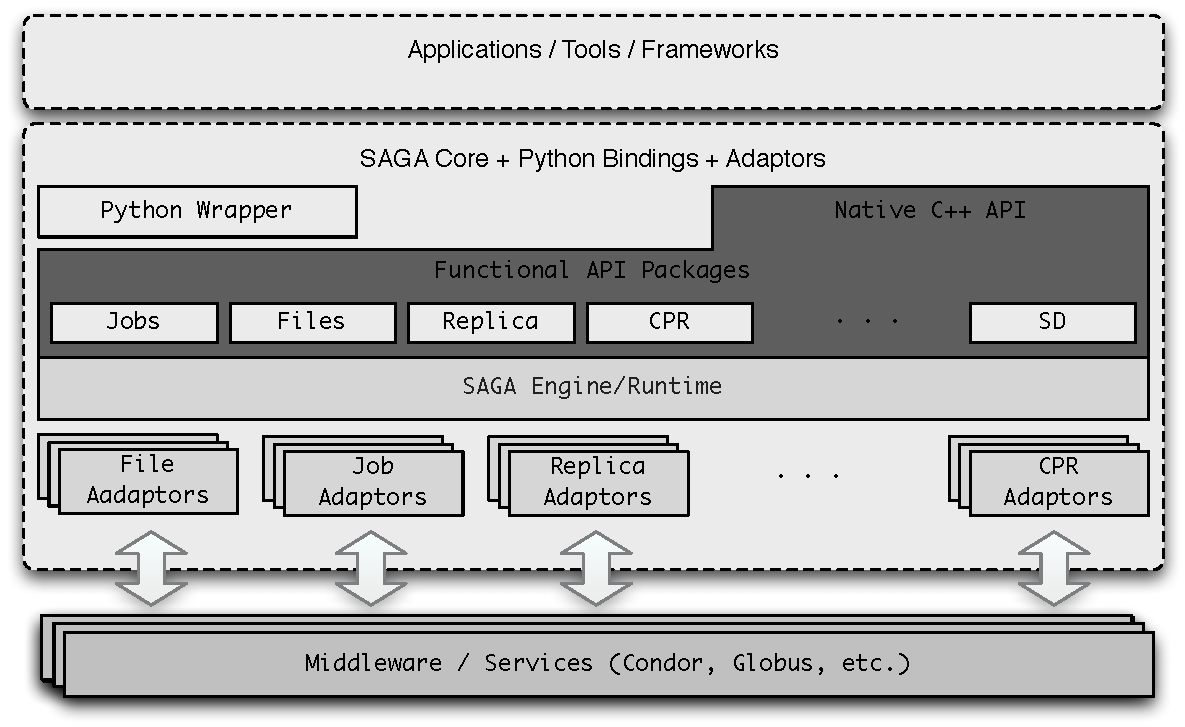
\includegraphics[width=1.0\textwidth]{./figures/figure_02}
    \caption{\footnotesize Layered schematic of the different components
    of SAGA.  Middleware specific adaptors make applications developed
    using SAGA portable.  Schematic showing the different ways in which
    SAGA can be used to develop distributed applications. (i) Using
    native SAGA calls to implement distributed functionality; (ii)
    Through the use of frameworks which provide either application-level
    usage modes, patterns and thus shielding the application from
    directly interfacing with the infrastructure.} \label{sagalayer}
\end{figure}
	
	
\subsection{API Specification}	

    A set of application groups expressed the desire for a simple
    programmatic interface that would be widely-adopted and
    widely-available, which led to the need and role for the SAGA API.
    The goal of such an interface is to provide a ``distributed
    computing counterpart to MPI'' (in impact if not in details), and to
    supply developers with a simple, uniform, and standard programmatic
    interface with which to develop applications.  Thanks to the efforts
    of many contributors, an initial specification of such an interface
    was released in 2008: the Simple API for Grid Applications
    (OGF-GFD-90). The scope and requirements of the SAGA API have been
    formally defined by OGF's SAGA Research Group (SAGA-RG). The SAGA-RG
    collected use cases from a broad user community and published them
    as OGF-GFD.70. The requirements and design for the SAGA API were
    directly derived from these use cases; this process has been
    documented and published in OGF-GFD.71. The end result of this
    process is the 1.0 version of the SAGA core specification
    (OGF-GFD.90), which defines language-independent syntax and
    semantics for the SAGA core API (error handling, session and context
    management, permissions, monitoring, attribute and task model) and
    functional packages (jobs, name-spaces, files, replicas, streams,
    RPC). Several API extension, such as CPR (OGF-GWD-R.96), Adverts
    (GFD-R-P.XX~), and Messaging (GWD-R.94) are currently under
    development and follow a similar, well-defined community-driven
    standardization and approval process. SAGA is now an Open Grid Forum
    (OGF) proposed recommendation on the path to becoming a standard. 
    The standardization is important because it makes it more likely
    that infrastructures will support SAGA, which may make it widely
    available for users of most national CI projects.
	
\subsection{C++/Python Implementation}

    The SAGA implementation referred to in this document is a reference
    implementation of the SAGA API specification written in C++. It is
    under active development by our group at the Center for Computation
    and Technology at Louisiana State University with many contributions
    from external groups and collaborators and strives to implement the
    complete set of functional API packages as defined in OGF-GFD-90
    while focusing on maximum practical relevance by providing
    middleware-bindings (Adaptors) for as many distributed middleware
    services as possible.

    SAGA is open source software, released under the Boost Software
    License. As shown in Figure \ref{sagalayer}, SAGA can be divided
    into three major components : (1) the \I{Core Components} which
    provide the API functionality, (2) the \I{Adaptors} which translate
    API calls into native middleware calls, and the (3) the Python API
    \I{Language Bindings} - a thin Python layer on top of the native C++
    API. The SAGA \I{Core Components} are a collection of dynamic
    libraries and header files that represent the functional API
    packages (see section 2.1) along with a lightweight,
    highly-configurable \I{Runtime} that manages call dispatching and
    the dynamic runtime loading of the \I{Middleware Adaptors}.

    \textbf{More information about SAGA can be found on the
    website: \\ \textit{http://saga.cct.lsu.edu}}

\subsection{SAGA Middleware Adaptors}

    The following list gives an overview of the currently available SAGA
    middleware adaptors, their development status and the functional API
    package they're interfacing.
    
    \textbf{TODO OLE: Copy list from website}
    
    
\subsection{SAGA-based Applications, Tools and Frameworks}
    
    \textbf{TODO SHANTENU: Add some stuff here. Esp. BigJob since it is important
    in the context of this work.} 
	
In the absence of a formal theoretical taxonomy of distributed
applications, % Fig.~\ref{Fig:sagaapps} can act a guide.  Using this
% classification system,
we use an informal classification system in there are three types of
distributed applications: (i) Applications where local functionality
is swapped for distributed functionality, or where distributed
execution modes are provided.  A simple but illustrative example is an
application that uses distributed resources for bulk submission. Here,
the application remains unchanged and even unaware of its distributed
execution, and the staging, coordination, and management are done by
external tools or agents. Most applications in this category are
classified as implicitly distributed.  (ii) Applications that are
naturally decomposable or have multiple components are then aggregated
or coordinated by some unifying or explicit mechanism.  DAG-based
workflows are probably the most common example of applications in this
category. Also, in this category, are applications that remain
unchanged but are enabled to utilize tools and services that provide
them the ability to utilize distributed resources.  Applications that
use Pilot Jobs to submit to multiple distributed resources also fall
in this category.  Finally, (iii) applications that are developed
using frameworks, where a framework is a generic name for a
development tool that supports specific application characteristics
(e.g. hierarchical job submission), and recurring patterns
(e.g. MapReduce, data parallelism) and system functionality.

% Lazarus~\cite{enkf-gmac09} provides several autonomic features, such
% as fault tolerance and dynamic resource selection, specifically for
% Ensemble-Kalman-Filter application scenarios.  SAGA has been used to
% develop system-level tools and applications for each of these types.

It is important to note that SAGA provides the basic API to implement
distributed functionality required by applications (typically used
directly by the first category of applications), and is also used to
implement higher-level APIs, abstractions, and frameworks that, in
turn, support the development, deployment and execution of distributed
applications~\cite{enkf-gmac09}. Merzky et\,al.~\cite{sagamontage09}
discusses how SAGA was used to implement a higher-level API to support
workflows. In this paper, we will discuss how SAGA can be used to
implement runtime frameworks to support the efficient execution of the
distributed applications.

\subsubsection{BigJob: A SAGA-based Pilot-Job Implementation:}

\emph{BigJob} is a SAGA-based Pilot-Job implementation. In contrast to
other Pilot-Job implementations, e.g., Falkon, BigJob natively
supports parallel applications (e.g. based on MPI) and works
independent of the underlying Grid infrastructure across different
heterogeneous backend, e.\,g.\ Grids and Cloud, reflecting the
advantage of using a SAGA-based approach. Further, the framework is
extensible and provides several hooks that can be used to support
other resource types and Pilot-Job frameworks.

% As shown in Figure~\ref{fig:figures_distributed_pilot_job}, BigJob currently
% provides a unified abstraction to Grids, Condor pools and
% Clouds. 
Using the same API, applications can dynamically allocate resources
via the big-job interface and bind sub-jobs to these resources.  We
describe how SAGA interfaces to different backends, while exposing the
same user-level BigJob interface and semantics.  A tutorial that
describes the BigJob API can be found at~\cite{bigjob_cloud_tutorial}.

\begin{figure}[ht]
    \centering
    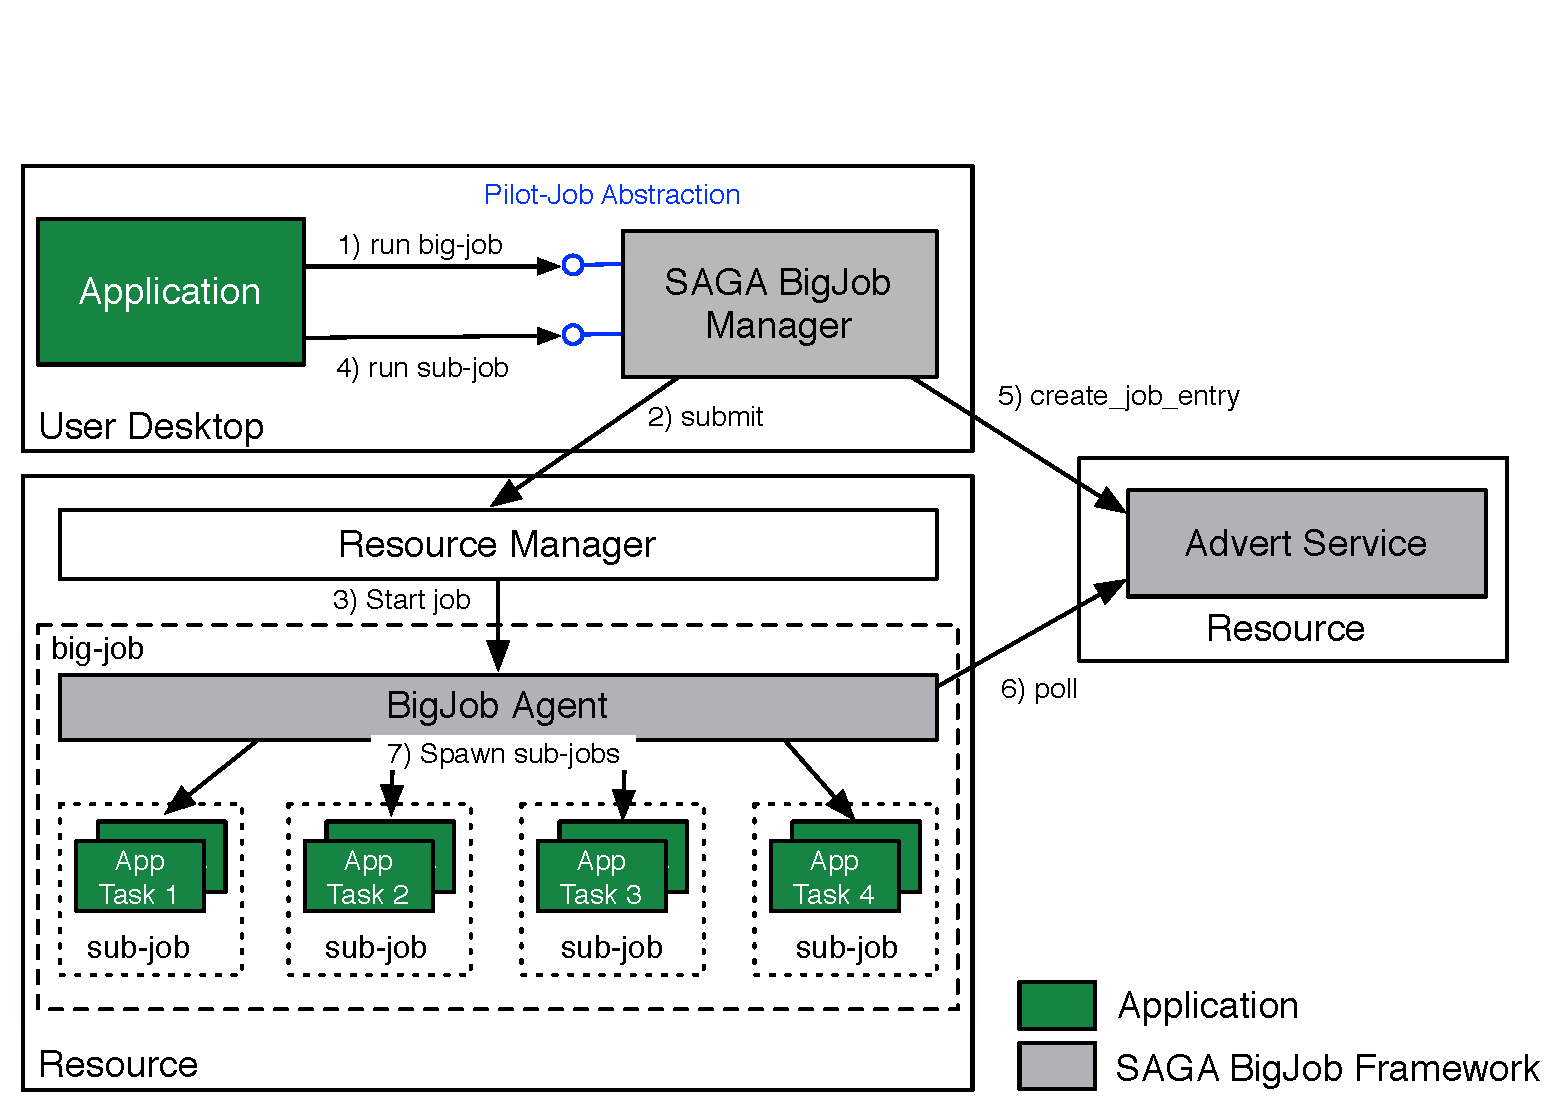
\includegraphics[width=0.45\textwidth]{figures/bigjob}
    \caption{BigJob Architecture: The core of the framework, the
      BigJob Manager, orchestrates a set of sub-jobs via a BigJob
      Agent using the SAGA job and file APIs.  The BigJob Agent is
      responsible for managing and monitoring sub-jobs.\up}
   \label{fig:figures_bigjob}
\end{figure}

\vspace{0.1in}
Figure~\ref{fig:figures_bigjob} shows an overview of the SAGA BigJob
implementation for computational Grids. The Grid BigJob comprises of
three components: (i) the BigJob Manager that provides the Pilot-Job
abstraction and manages the orchestration and scheduling of BigJobs
(which in turn allows the management of both big-job objects and
sub-jobs), (ii) the BigJob Agent that represents the pilot job and
thus, the application-level resource manager on the respective
resource, and (iii) advert service which is used for communication
between the BigJob Manager and Agent.


\pagebreak	
\section {Condor}

    Condor is an open source high-throughput computing software
    framework for coarse-grained distributed parallelization of
    computationally intensive tasks. Condor can be used to manage
    workload on a dedicated cluster of computers, and/or to farm out
    work to idle desktop computers. Condor is developed by the Condor
    team at the University of Wisconsin–Madison and is licensed under
    the Apache License 2.0.
    
    Condor provides a SOAP web-service API called \textit{BirdBath}
    \footnote{\texttt{http://www.cs.wisc.edu/condor/birdbath/}}, which
    can be used to submit, control and monitor jobs. BirdBath is part of
    the standard Condor distribution, but it has to be enabled
    explicitly on the server side. The far more common usage mode of
    Condor is through the condor command line tools. Since they are
    available on all Condor systems, they seem to be the better
    candidate for a generic interface to SAGA.
	
    \textbf{More information about Condor can be found on the
    website: \\ \textit{http://www.cs.wisc.edu/condor/}}
	
	
\subsection{Condor-G}

    \begin{wrapfigure}{l}{0.5\textwidth}
    \vspace{-30pt}
        \begin{center}
        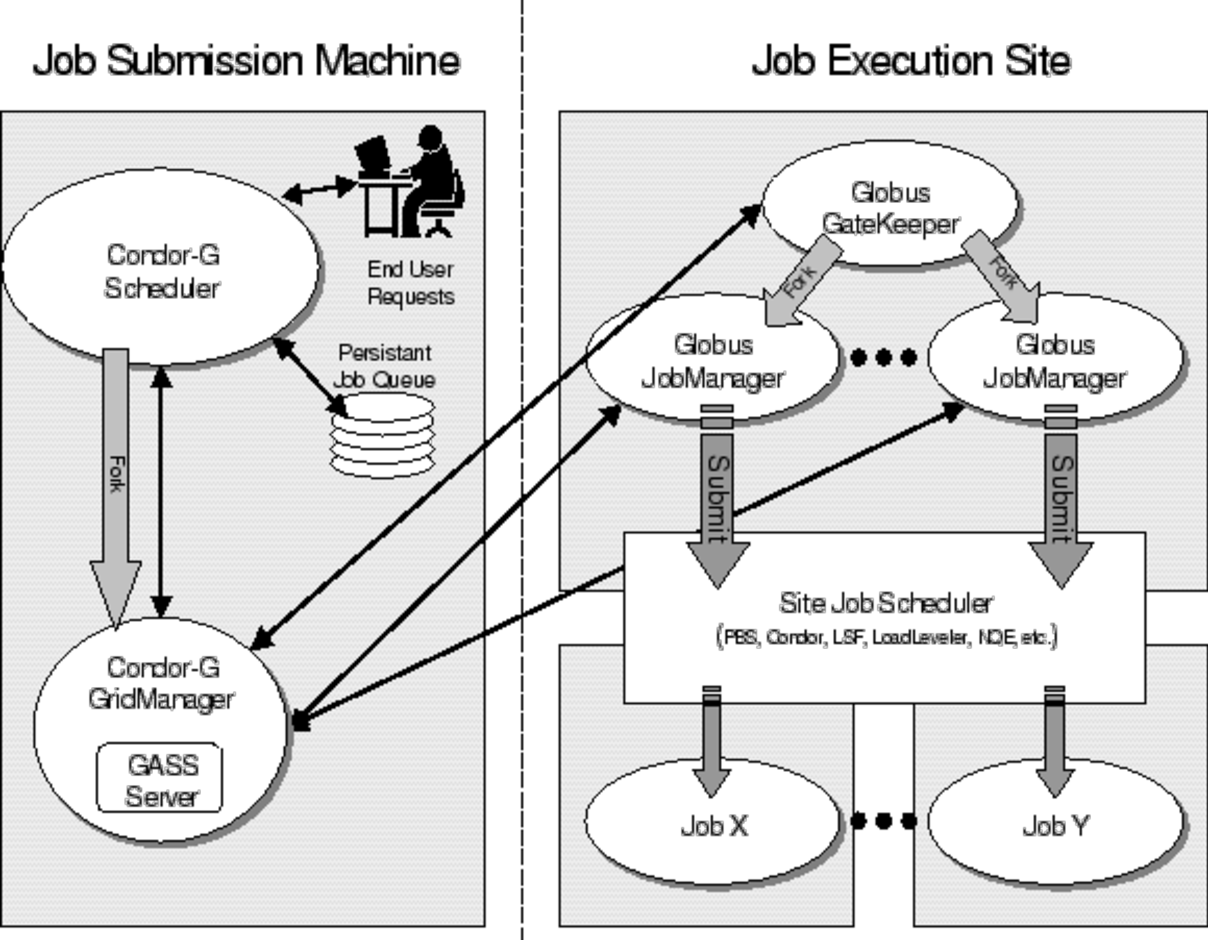
\includegraphics[width=0.5\textwidth]{./figures/condor_g}
        \end{center}
        \vspace{-20pt}
        \caption{\footnotesize Remote Execution by Condor-G on Globus managed resources. (Image taken from the Condor manual)} 
        \vspace{-22pt}
    \end{wrapfigure}
    
    Condor-G allows Condor jobs to use resources not under its direct
    control. It is mostly used to talk to Grid and Cloud resources, like
    pre-WS and WS Globus, Nordugrid ARC, UNICORE and Amazon EC2. But it
    can also be used to talk to other batch systems, like Torque/PBS and
    LSF. Condor-G is a "plugin" for Condor that allows the user to use
    the familiar Condor command line utilities  (e.g. condor\_submit,
    condor\_q) to submit jobs to a Globus resource.\\[1em]
   
  
   
    \textbf{More information about Condor-G can be found on the
    website: \\ \textit{http://www.cs.wisc.edu/condor/condorg/}}
   
   \vfill % footnote
    


    
	
\subsection{Condor Glide-in}

    Glide-in allows a user to temporarily extend a condor pool with
    additional resources that are not managed by condor but by globus.
    This is being achieved by submitting and executing a condor\_startd
    executable (which is also running on every 'regular' condor
    resource) along with the right parameters through the Globus
    resource manager (GRAM). The submission is done via Condor-G, but
    could in principle also be done via another method.

    \textbf{More information about Condor-G can be found on the
    website: \\ \textit{http://www.cs.wisc.edu/condor/condorg/}}

\pagebreak

\section {Integration}

\subsection{Use-Cases}
These are the use-cases that have been identified within the ExTENCI project. The
final outcome of this integration project will be tested against these use-cases
to make sure that the implementation is feature-complete.

\begin{itemize}
\item \textbf{U.01:} A user submits, monitors and controls Condor jobs through
the SAGA Job API.

\item \textbf{U.02:} A user can select Condor-G ("Globus via Condor") resources
as well as regular Condor pools for job execution through the SAGA Job API.

\item \textbf{U.03:}

\end{itemize}

\subsection{Requirements}

In addition to the use-cases, we define a set of requirements that the 
implementation has to fulfill:

\begin{itemize}
\item \textbf{R.01:} E.g. stuff like types of system where this has to work, etc.
\end{itemize}

\subsection{Adaptor Architecture}

\begin{figure}
  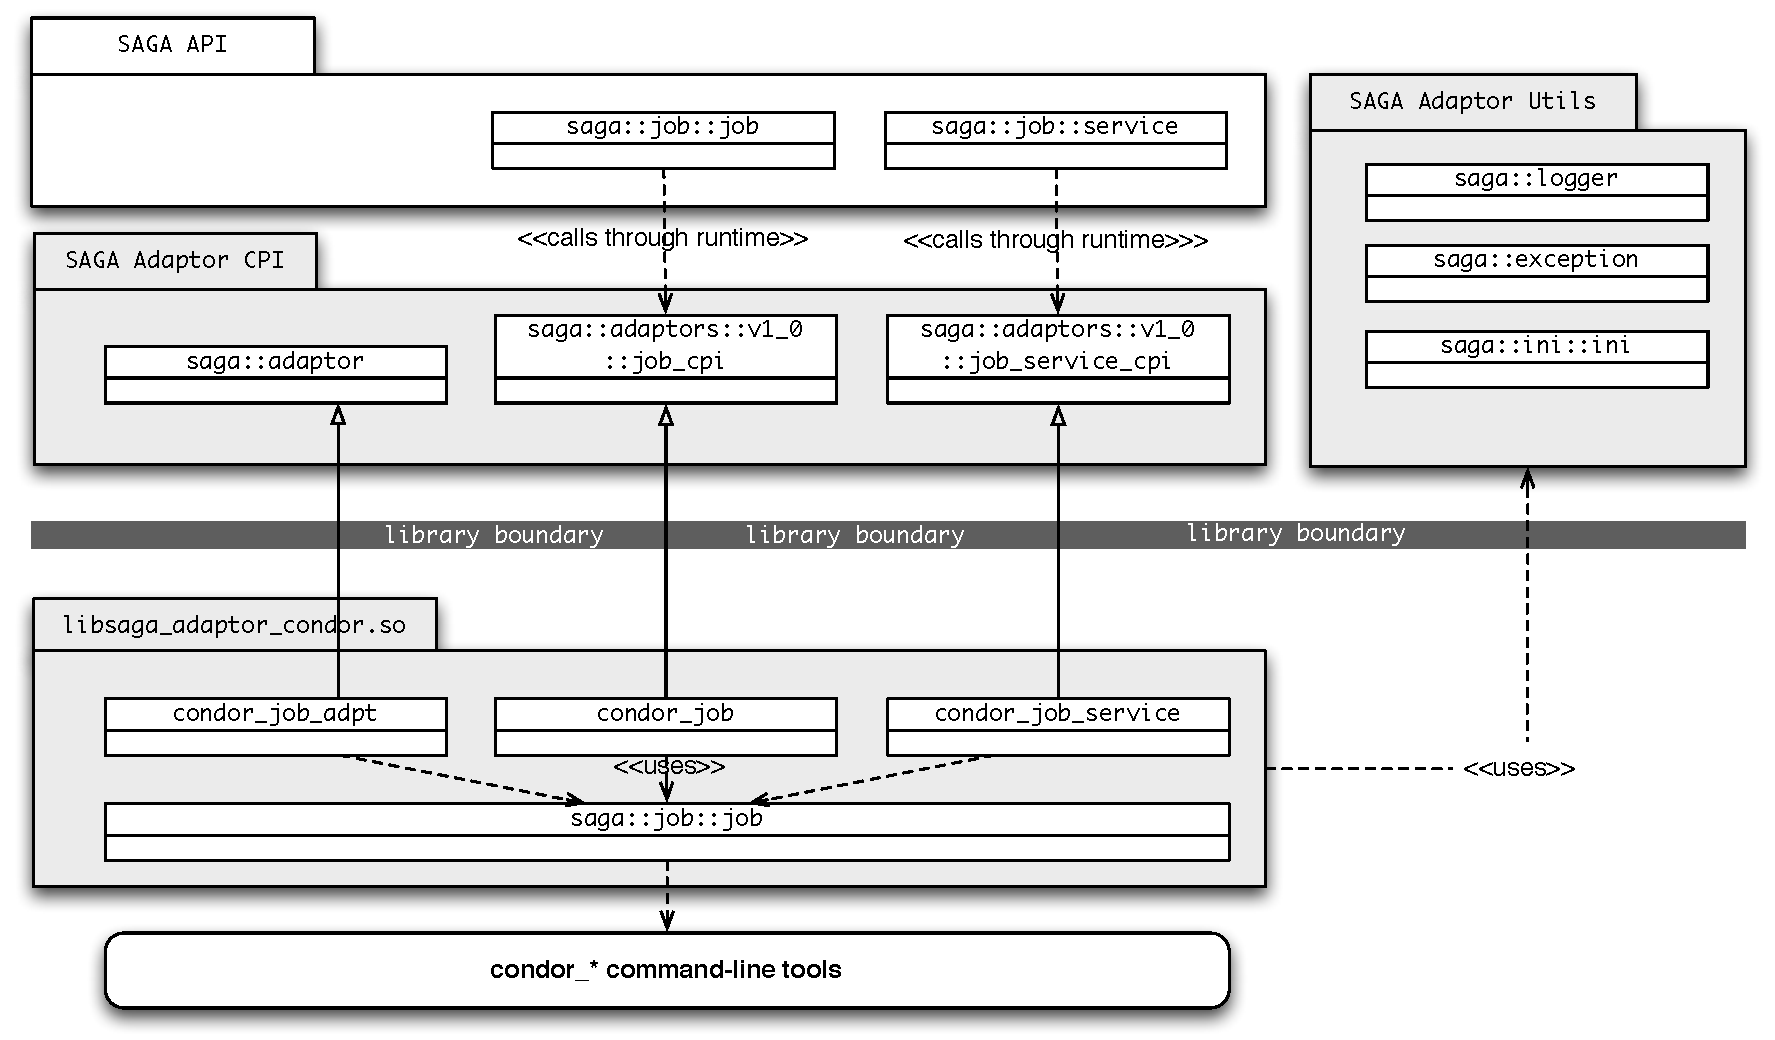
\includegraphics[width=1.0\textwidth]{./figures/condor_adaptor_arch}
  \caption{\footnotesize The SAGA Condor adaptor architecture. The adaptor interfaces
  with SAGA's well defined Capability Provider Interface (CPI), or \textit{Adaptor API}.
  This ensures that the adaptor fully integrates with SAGA's intelligent adaptor selection
  mechanism, logging and error handling facilities. To ensure maximum versatility across
  platforms, the Condor adaptors uses the boost::process API to call the Condor command 
  line tools. }
  
%\vspace{-1em}
\label{adaptor_arch}
\end{figure}

\bibliographystyle{unsrt}
\bibliography{saga}
\end{document}


